


\section{哈希函数简述}
% \subsection{定义与性质}

给定一个任意长度的消息$M$,哈希函数$H$能够将$M$映射为固定长度$n$bit的哈希值$h=H(M)$。在SHA-1中为160bit,在MD5
中为128bit。
哈希函数具有以下三个基本性质\cite{kelsey2005second}:
\begin{itemize}
    \item 抗原像攻击。对于给定的哈希值$Y$,攻击者无法在少于$2^n$次的计算下找到输入消息$X$,满足$Y=H(X)$。
    \item 抗第二原像攻击。对于给定的一个消息$M$,攻击者无法在少于$2^n$次的计算下找到另一个消息$M^\prime$使得$H(M^\prime) = H(M)$。
    \item 抗碰撞攻击。攻击者无法在少于$2^{n/2}$次的计算下找到任意两个消息$M$和$M^\prime$,$M\neq M^\prime$且$H(M)=H(M^\prime)$。
\end{itemize}

如果找到一种方法,能够破坏上面任何一种性质,就可以说是攻破了该哈希函数。
这个寻找的过程,就被称为攻击\textit{Attack}或者密码分析\textit{Cryptanalysis}。

\section{攻击进展}

在1998年的国际密码学会上,Chabaud和Joux提出一种对SHA-0的攻击方式\cite{10.1007/BFb0055720}:在$2^{61}$的计算复杂度之内,就可以发现一次碰撞(即两个不同的消息对应到相同的消息摘要);这个数字小于生日攻击法所需的$2^{80}$,也就是说,存在一种算法,使其安全性不到一个理想的散列函数抵抗攻击所应具备的计算复杂度。

2004年8月12日,Joux, Carribault, Lemuet和Jalby宣布找到SHA-0算法的完整碰撞的方法,这是归纳Chabaud和Joux的攻击所完成的结果。发现一个完整碰撞只需要$2^{51}$的计算复杂度。他们使用的是一台有256颗Itanium2处理器的超级电脑,约耗80,000 CPU时间。

2004年8月17日,在CRYPTO大会上,王小云,冯登国(Feng)、来学嘉(Lai),和于红波(Yu)宣布了攻击MD5、SHA-0和其他散列函数的初步结果。他们攻击SHA-0的计算复杂度是$2^{40}$,这意味的他们的攻击成果比Joux还有其他人所做的更好。

2005年,Rijmen和Oswald发表了对SHA-1较弱版本(53次的加密循环而非80次)的攻击\cite{cryptoeprint:2005:010}:在$2^{80}$的计算复杂度之内找到碰撞。

2005年二月,王小云、殷益群及于红波发表了对完整版SHA-1的攻击\cite{wang2005finding},只需少于$2^{69}$的计算复杂度,就能找到一组碰撞。

2005年8月17日的CRYPTO会议尾声中王小云、姚期智、姚储枫再度发表更有效率的SHA-1攻击法,能在$2^{63}$的计算复杂度内找到碰撞。

2006年的CRYPTO会议上,Christian Rechberger和Christophe De Cannière宣布他们能在容许攻击者决定部分原消息的条件之下,找到SHA-1的一个碰撞\cite{10.1007/11935230_1}。

在密码学的理论中,任何攻击方式,其计算复杂度若少于暴力搜索法所需要的计算复杂度,就能被视为针对该密码系统的一种破密法;但这并不表示该破密法已经可以进入实际应用的阶段。上述各种攻击均在理论上指出了SHA-1的不安全,并且给出了实际的碰撞,但是这种碰撞是随机的,如何给出真实意义上具备威胁的攻击,也是
一个研究的难题。

在2011年,NIST废除了SHA-1,其不再是安全哈希算法的标准。Google、Microsoft、Google以及Mozilla它们旗下的浏览器将在2017年停止接受使用SHA-1算法签名的SSL证书。

2017年2月23日,Google宣称他们与CWI Amsterdam合作共同创建了两个有着相同的SHA-1值但内容不同的PDF文件\cite{stevens2017first},这代表SHA-1算法已被正式攻破。

2020年,来自法国和新加坡南洋理工大学的研究人员Gaëtan Leurent和Thomas Peyrin使用SHA-1选择前缀碰撞制造了一次针对PGP协议的攻击\cite{leurent2020sha},该攻击仅仅消耗了900块GTX1060 GPU 1个月的时间。这表明使用SHA-1签名的网络协议已经几乎无法提供任何安全性,使用更安全的SHA-2或SHA-3替换SHA-1已经变得十分紧迫。


\section{攻击算法}

针对SHA-1等哈希函数的密码分析算法,主要有以王小云院士的一系列工作为代表的差分密码分析法(Differential cryptanalysis)和以
Marc Steven所提出的选择前缀碰撞(\textit{chosen-prefix} collision\cite{stevens2007chosen})攻击法。

\subsection{差分密码分析}

差分密码分析是一种经典的密码分析方法,其不单可以用来分析哈希函数,还可以用来分析分组密码、流密码等,通常是选择明文攻击。
该分析方法的具体实施与要分析的加密或哈希算法相关。

给定两个消息(明文)$M$和$M’$,可以计算$H(M)$与$H(M’)$,进一步可以计算明文差异与密码差异$\Delta M=M \oplus M’, \Delta H=H(M) \oplus H(M’)$,明文差异与密文差异构成的差异对$(\Delta M, \Delta H)$被称为一个差分。$\oplus$是计算差分的符号,通常使用异或XOR。

在差分分析中,还有一个很重要的概念是差分路径。如果$\Delta H=0$则被碰撞发生(有可能是局部碰撞),一系列局部碰撞构成的路径称为差分路径\cite{wang2005finding}。

差分分析在密码分析中是一种强有力的理论分析方法,绝大部分的密码分析工作都会使用这种分析方法,其思想是分析改变输入并最终输入的改变对输出造成的影响,
进而得到加密系统(或哈希函数)的缺陷,其具体实施也需要较为深厚的数学知识甚至是直觉。以下列举一些应用该分析方法到哈希函数攻击上重要的思想,其图示可见\ref{fig:diff}:

\begin{figure}[h]
    \centering
    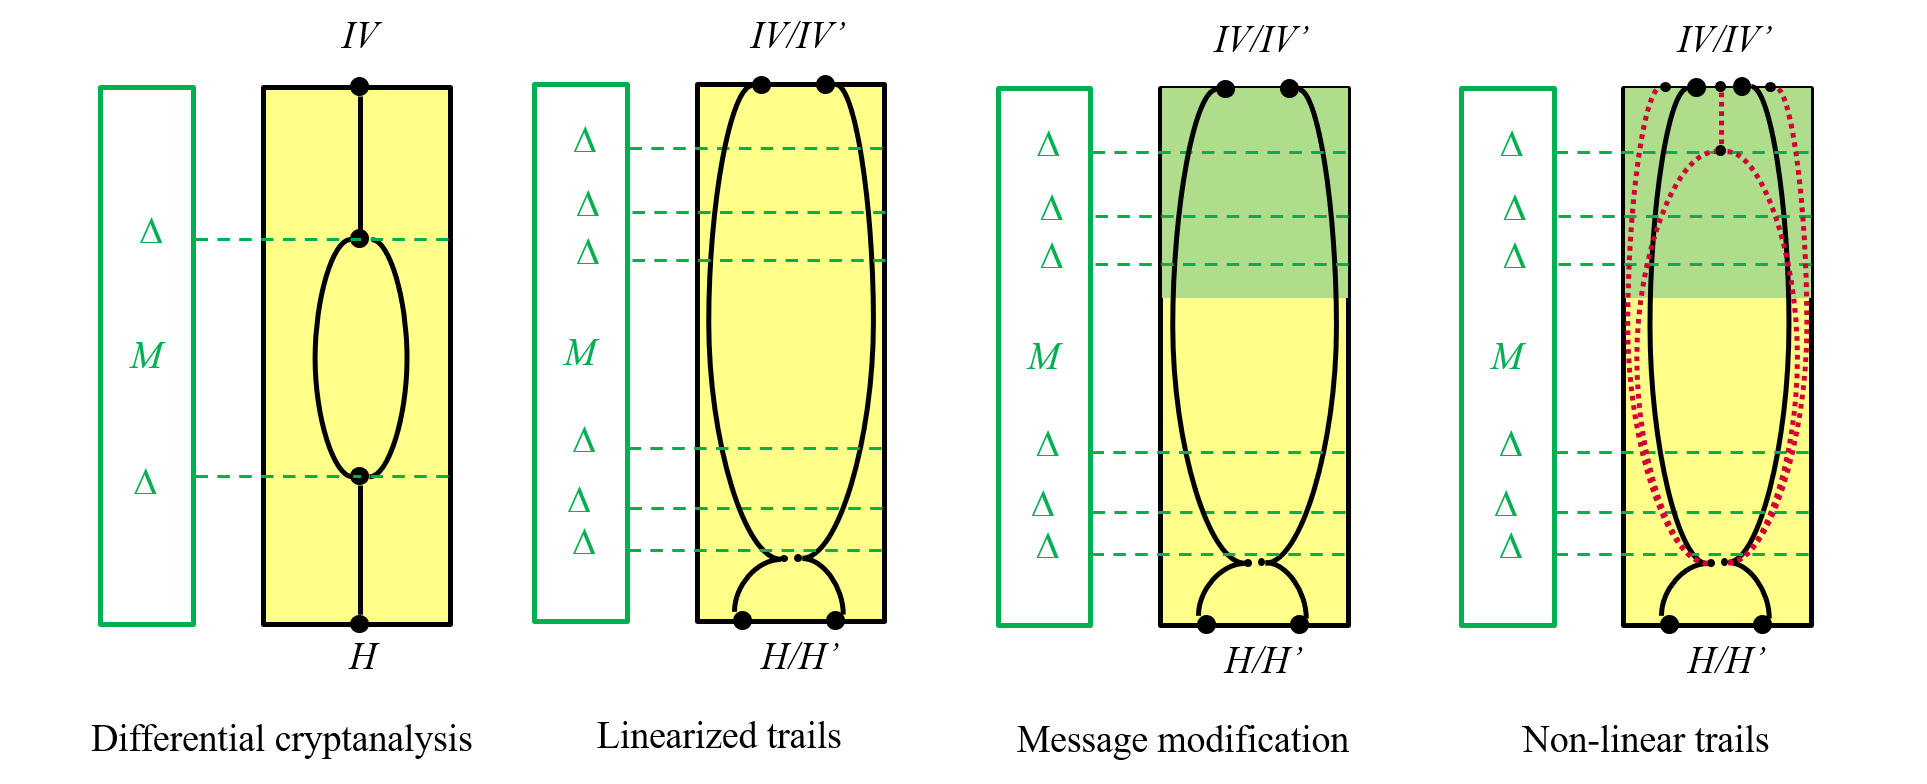
\includegraphics[width=0.85\linewidth]{differential.png}
    \caption{差分密码分析中常用的分析方法}
    \label{fig:diff}
\end{figure}

\begin{itemize}
    \item \textbf{线性化(Linearization\cite{chabaud1998differential})}。使用一个线性步骤函数来构建一个具备高碰撞概率的差分路径。带有较低权重(指的是汉明距离)的输出差分$\Delta M$可以用来在压缩函数中找到一个临近碰撞。
    \item \textbf{消息修改(Message modification \cite{biham2004near}\cite{wang2005finding})}。在一个针对哈希函数的差分分析中,由于没有密钥,攻击者可以选择直接满足一些路径约束的消息。
    \item \textbf{非线性轨迹追踪(Non-linear trails \cite{wang2005finding})}。为了得到更灵活的差分路径,前几步可以使用非线性函数,而不需要受线性步骤函数的约束。这种方法不会影响搜索满足要求的消息的复杂度,但是使得从任意输入差分构建路径到到固定长度的输出差分。
    \item \textbf{多块碰撞技术(Multi-block technique \cite{chabaud1998differential}\cite{wang2005finding})}。多块碰撞技术利用了压缩函数中的Davies-Meyer构造性质。实际上,它可以被写成$h(x, m)=x + E_m(x)$,这里$E$指的是分组密码,$+$指的是一些组操作。
\end{itemize}

\subsection{选择前缀碰撞}

上面提到,差分密码分析是分析哈希函数性质的重要理论工具。而选择前缀碰撞\cite{stevens2007chosen}使得对哈希函数
的碰撞攻击变得真正对现实应用具备威胁性。

一个常规的碰撞攻击从一个初始化向量$IV$开始,经过一系列运算后在$C_1$和$C_2$处发生碰撞。这种
攻击的问题是造成碰撞的$C_1$和$C_2$通常是随机的。要使得这种攻击方法更具威胁性,可以在
文件中藏入一些会被忽视掉的信息,比如注释。

而如果可以在$IV$之后添加一个相同的前缀\textit{prefix}和后缀\textit{suffix},这样对于消息的可操作性
更强,而且通常来说不会增加计算复杂度,可见图\ref{fig:chosen}左侧。对于产生碰撞的消息不是\textit{meaningful}的问题,使用该方法后,可以在
许多支持条件分支语句的文件格式中,添加有含义的前缀,进而造成攻击。在2017年谷歌和CWI发布了
两个具有不同颜色、相同文字信息、相同SHA-1哈希值的PDF文档\cite{stevens2017first},其攻击策略就是采用了这种方法。通过条件分支语句,使得PDF文件中包含两种不同的图片。这种针对PDF文档的攻击方式已经十分常见,作者在github上开放了
简易的工具实现这种攻击,可以在很短的(一页不到1秒)时间内对任意PDF文档实现碰撞攻击。

尽管有了这种添加前缀和后缀的攻击方式,但是网络世界中的安全协议通常是更加复杂的,需要更有效的方式来进行攻击。这种方式就是选择前缀碰撞。其图示可见\ref{fig:chosen}。这里对在$IV$后添加的前缀不加限制,
可以是假设分别是$P_1$和$P_2$,然后通过一系列的中间运算,最终得到碰撞。

使用相同前缀碰撞可以破坏完整性,理论上可以破坏数字签名。而使用选择前缀碰撞,可以破坏密钥认证,破坏TLS、LKE和SSH
等网络协议。
\begin{figure}[h]
    \centering
    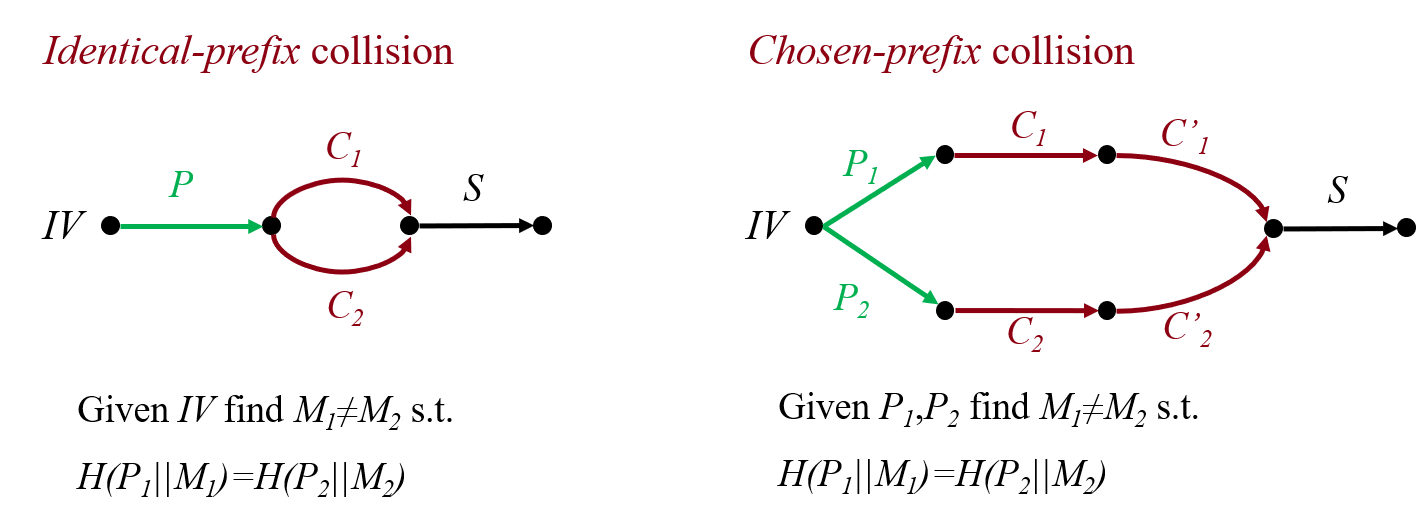
\includegraphics[width=0.75\linewidth]{chosen.png}
    \caption{相同前缀碰撞与选择前缀碰撞}
    \label{fig:chosen}
\end{figure}


通常来说,选择前缀碰撞比相同前缀碰撞有着更大的计算复杂性,但是存在一定的方法将相同前缀碰撞转换成选择前缀碰撞。


下面给出一个使用选择前缀碰撞造成身份冒充攻击的例子:

首先\textit{Alice}有一个文件,首先她生成她的公钥$k_A$,然后使用公钥在PKI(Public Key Infrastructure)中生成签名,完成认证。

而\textit{Bob}想要冒充\textit{Alice},他需要准备两个文件,一个是\textit{Alice}的公钥和她的文档,这个都是
能够轻松得到。另外他需要准备一个自己的公钥$k_B$和一个文档,这个文档要能够与\textit{Bob}的公钥拼接起来产生碰撞,即满足$H(Alice||k_A)=H(Bob||k_B)$。\textit{Bob}要求CA认证他的公钥$k_B$,然后他
将自己的签名复制到\textit{Alice}的文档中,就成功地冒充了\textit{Alice}。

\section{SHA-1的现状}
首先,在2017年之后,大多数现代浏览器都会拒绝使用以SHA-1作为哈希函数的证书,Chrome、Firefox、Edge等。
但是SHA-1证书依然存在,在一些早期的应用程序中。
甚至还有一些CA还在卖SHA-1证书。
SHA-1证书依然会被一些非浏览器的TLS客户端接接受。
例如Windows 10邮件APP在使用SHA-1签名的证书连接时没有报错。
SHA-1的PGP签名依然被信任。
还有常用的软件Git,TLS 1.2握手,包括很多文档应用等依然使用SHA-1,这些都是目前依然存在
的安全隐患。尽管Linus指出Git中使用的SHA-1经过了增强,就是在输入SHA-1的文件中还加入了
文件的长度信息,但是理论上依然有很大人为地制造碰撞的空间,因此构造两个相同SHA-1的commit是可行的。

\bibliography{report1}